\documentclass[border=16pt]{standalone}
\usepackage[T1]{fontenc}
\usepackage{helvet}
\renewcommand{\familydefault}{\sfdefault}
\usepackage{tikz}
\usetikzlibrary{positioning,arrows.meta,calc,fit,backgrounds}

\definecolor{clsBlue}{HTML}{2C5AA0}
\definecolor{ownGreen}{HTML}{1F7A5A}
\definecolor{ownBg}{HTML}{E4F3EC}
\definecolor{viewOr}{HTML}{C4600A}
\definecolor{viewBg}{HTML}{FCEBD7}
\definecolor{topoBg}{HTML}{E1E1E1}
\definecolor{physBand}{HTML}{CFE6CB}

\begin{document}
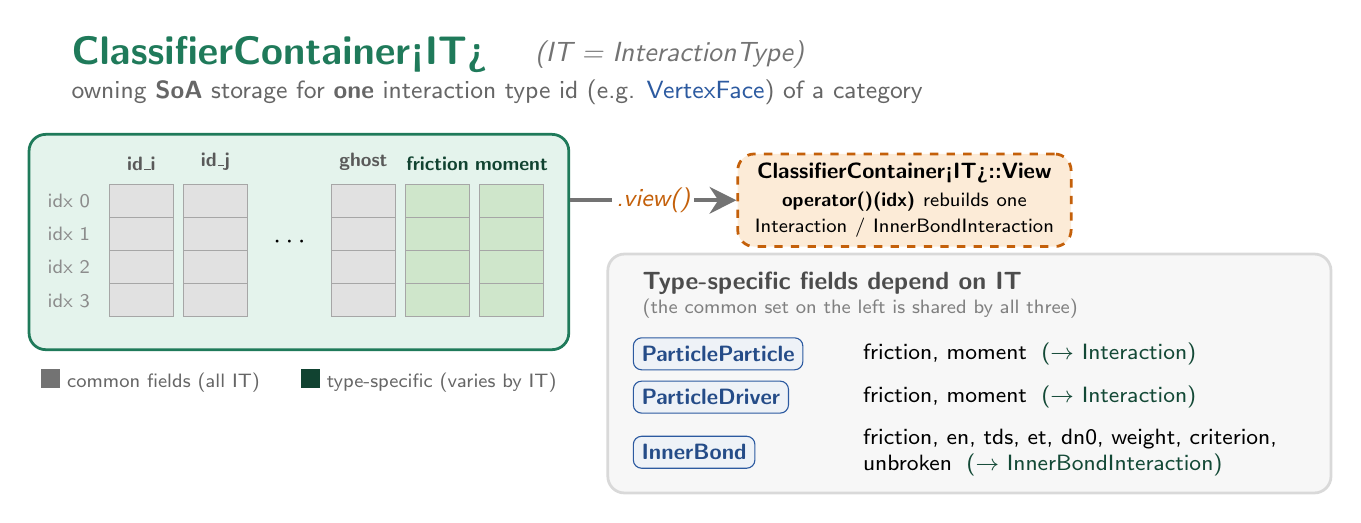
\begin{tikzpicture}[
  font=\sffamily,
  >=Stealth,
  bx/.style={rounded corners=6pt, line width=1pt},
  flow/.style={-{Stealth[length=3.4mm,width=3.4mm]}, line width=1.4pt, draw=black!55},
  itpill/.style={rounded corners=3pt, draw=clsBlue, fill=clsBlue!8, font=\sffamily\footnotesize\bfseries, text=clsBlue!85!black, inner sep=3pt},
]

% ===================== TITLE =====================
\node[anchor=west, font=\sffamily\Large\bfseries, text=ownGreen] (ttl) at (0,4.2){ClassifierContainer<IT>};
\node[anchor=west, font=\sffamily\normalsize\itshape, text=black!55] at ($(ttl.east)+(0.35,0)$){(IT = InteractionType)};
\node[anchor=west, font=\sffamily\small, text=black!60] at (0,3.72)
  {owning \textbf{SoA} storage for \textbf{one} interaction type id (e.g. \textcolor{clsBlue}{VertexFace}) of a category};

% ===================== LEFT : SoA container =====================
\def\cw{0.82}\def\ch{0.42}\def\cg{0.12}
\def\x0{0.6}\def\ytop{2.55}
\foreach \c/\fll in {0/topoBg,1/topoBg,3/topoBg,4/physBand,5/physBand}{
  \pgfmathsetmacro\xx{\x0+\c*(\cw+\cg)}
  \foreach \r in {0,1,2,3}{
    \pgfmathsetmacro\yy{\ytop-\r*\ch}
    \fill[\fll,draw=black!35,line width=0.4pt] ({\xx},{\yy}) rectangle ({\xx+\cw},{\yy-\ch});}}
\node at ({\x0+2*(\cw+\cg)+0.5*\cw},{\ytop-2*\ch+0.1}){$\cdots$};
\foreach \c/\lbl/\col in {0/{id\_i}/black!65, 1/{id\_j}/black!65, 3/{ghost}/black!65, 4/{friction}/ownGreen!55!black, 5/{moment}/ownGreen!55!black}{
  \pgfmathsetmacro\xc{\x0+\c*(\cw+\cg)+0.5*\cw}
  \node[font=\sffamily\scriptsize\bfseries, text=\col, anchor=south] at ({\xc},{\ytop+0.06}){\lbl};}
\foreach \r in {0,1,2,3}{
  \pgfmathsetmacro\yy{\ytop-\r*\ch-0.5*\ch}
  \node[font=\sffamily\scriptsize, text=black!45, anchor=east] at ({\x0-0.12},{\yy}){idx \r};}
\coordinate (cTL) at ({\x0-0.9},{\ytop+0.52});
\coordinate (cBR) at ({\x0+5*(\cw+\cg)+\cw+0.2},{\ytop-4*\ch-0.3});
\begin{scope}[on background layer]
  \node[bx, draw=ownGreen, fill=ownBg, fit={(cTL)(cBR)}] (cbox){};
\end{scope}
\node[font=\sffamily\scriptsize, text=black!60, anchor=north west] at ($(cbox.south west)+(0.05,-0.10)$)
  {\textcolor{black!55}{\rule{2.4mm}{2.4mm}} common fields (all IT)\qquad
   \textcolor{ownGreen!55!black}{\rule{2.4mm}{2.4mm}} type-specific (varies by IT)};

% ===================== RIGHT-TOP : view() -> View =====================
\node[bx, draw=viewOr, dashed, fill=viewBg, font=\sffamily\footnotesize, align=center, text width=4.0cm]
  (view) at (10.7,2.35){\textbf{ClassifierContainer<IT>::View}\\[2pt]\scriptsize \textbf{operator()(idx)} rebuilds one\\ Interaction / InnerBondInteraction};
\draw[flow] (cbox.east|-view) -- node[font=\sffamily\small\itshape,text=viewOr,fill=white,inner sep=1.5pt]{.view()} (view.west);

% ===================== RIGHT-BOTTOM : specializations =====================
\begin{scope}[on background layer]
  \node[bx, draw=black!15, fill=black!3, fit={(7.05,1.55)(16.0,-1.25)}] {};
\end{scope}
\node[font=\sffamily\small\bfseries, text=black!70, anchor=west] at (7.25,1.3){Type-specific fields depend on IT};
\node[font=\sffamily\scriptsize, text=black!50, anchor=west] at (7.25,0.97){(the common set on the left is shared by all three)};

\node[itpill, anchor=west] at (7.25,0.4){ParticleParticle};
\node[font=\sffamily\footnotesize, anchor=west] at (10.05,0.4)
  {friction, moment \;\textcolor{ownGreen!60!black}{($\to$ Interaction)}};

\node[itpill, anchor=west] at (7.25,-0.15){ParticleDriver};
\node[font=\sffamily\footnotesize, anchor=west] at (10.05,-0.15)
  {friction, moment \;\textcolor{ownGreen!60!black}{($\to$ Interaction)}};

\node[itpill, anchor=west] at (7.25,-0.85){InnerBond};
\node[font=\sffamily\footnotesize, anchor=west, text width=5.7cm, align=left] at (10.05,-0.85)
  {friction, en, tds, et, dn0, weight, criterion, unbroken \;\textcolor{ownGreen!60!black}{($\to$ InnerBondInteraction)}};

\end{tikzpicture}
\end{document}